\section{Task 7: Defeating XSS Attacks Using CSP}
%

\begin{lstlisting}[caption=Inital CSP configuration by Apache.,
    label={lst:csp_config_init_apache}]
    # Purpose: Do not set CSP policies
    <VirtualHost *:80>
    DocumentRoot /var/www/csp
    ServerName www.example32a.com
    DirectoryIndex index.html
    </VirtualHost>
    # Purpose: Setting CSP policies in Apache configuration
    <VirtualHost *:80>
    DocumentRoot /var/www/csp
    ServerName www.example32b.com
    DirectoryIndex index.html
    Header set Content-Security-Policy " \
    default-src 'self'; \
    script-src 'self' *.example70.com \
    "
    </VirtualHost>
    # Purpose: Setting CSP policies in web applications
    <VirtualHost *:80>
    DocumentRoot /var/www/csp
    ServerName www.example32c.com
    DirectoryIndex phpindex.php
    </VirtualHost>    
\end{lstlisting}

\begin{lstlisting}[caption=Inital CSP configuration by web application,
    label={lst:csp_config_init_web}]
<?php
$cspheader = "Content-Security-Policy:".
"default-src 'self';".
"script-src 'self' 'nonce-111-111-111' *.example70.com".
"";
header($cspheader);
?>
<?php include 'index.html';?>
\end{lstlisting}

\textbf{1. Describe and explain your observations when you visit these websites.}\\
\textbf{2. Click the button in the web pages form all the three websites, describe and
explain your observations.}

\begin{itemize}
    \item \emph{example32a}: all Areas were OK and the button could trigger a pop-up window
    (see \autoref{fig:exampe_a_init}). All inline or external-linked scripts were executed
    successfully since there is not CSP policy set-up to \url{www.example32a.com}
    (see \autoref{lst:csp_config_init_apache}).
    \item \emph{example32b}: Areas 1, 2, 3, 5 were Failed; the button could not trigger a
    pop-up window (see \autoref{fig:example_b_init}). The reason is that CSP of \url{www.example32b.com} allowed scripts from
    the server itself and \url{*.example70.com}. CSP did not allow incline scripts
    (see \autoref{lst:csp_config_init_apache}).
    \item \emph{example32c}: Areas 2, 3, 5 were Failed; the button could not trigger a
    pop-up window (see \autoref{fig:example_c_init}). The reason is that CSP of
    \url{www.example32c.com} only allowed scripts from the server itself, \url{*.example70.com},
    and inline script having \emph{nonce=`111-111-111'} (see \autoref{lst:csp_config_init_web}).
\end{itemize}

\begin{figure}[h]
    \centering
    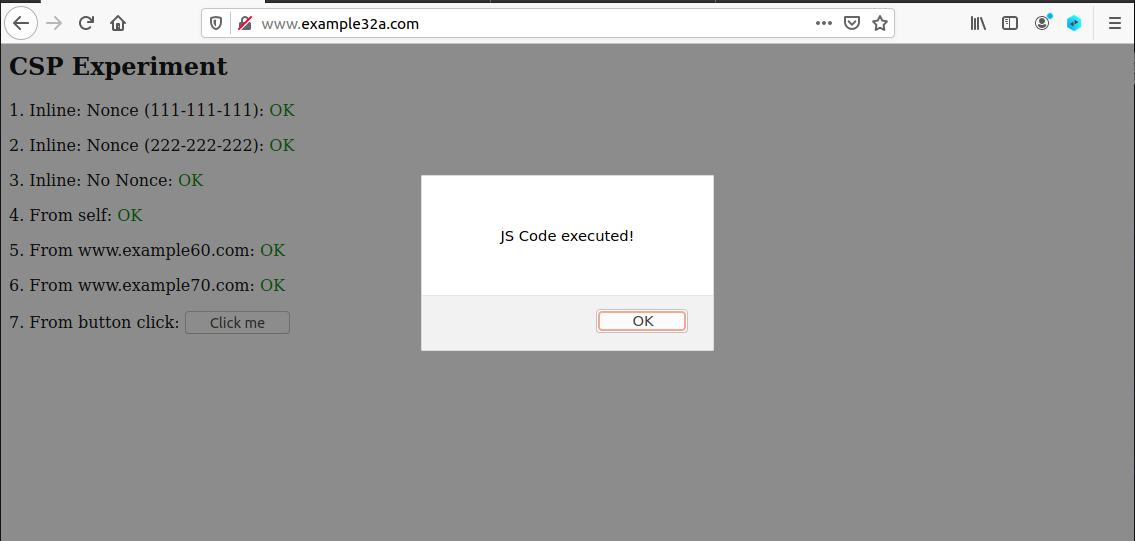
\includegraphics[height=\textheight,width=\textwidth,keepaspectratio]
    {figures/example_a_all_OK.png}
    \caption{\url{www.example32a.com} initial status.}
    \label{fig:exampe_a_init}
\end{figure}

\begin{figure}[h]
    \centering
    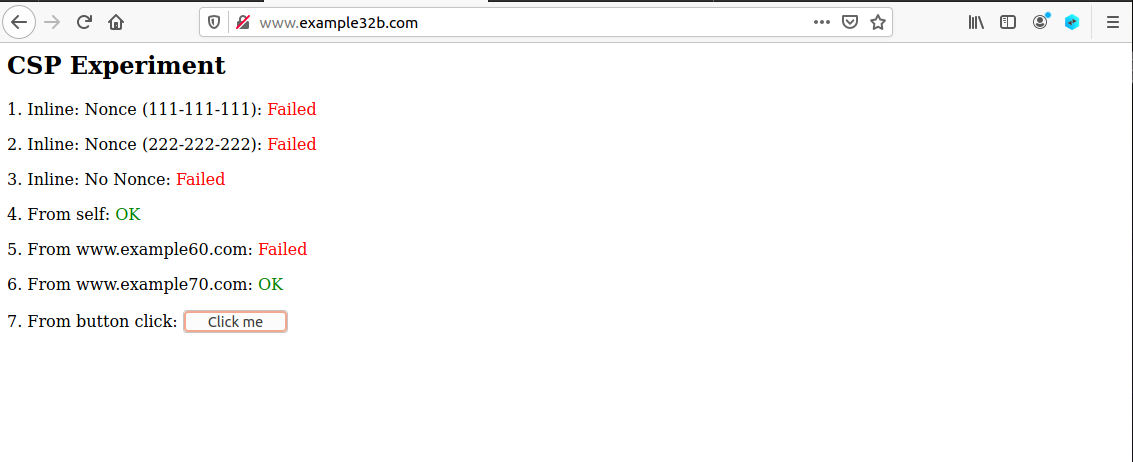
\includegraphics[height=\textheight,width=\textwidth,keepaspectratio]
    {figures/example_b_initial.png}
    \caption{\url{www.example32b.com} initial status.}
    \label{fig:example_b_init}
\end{figure}

\begin{figure}[h]
    \centering
    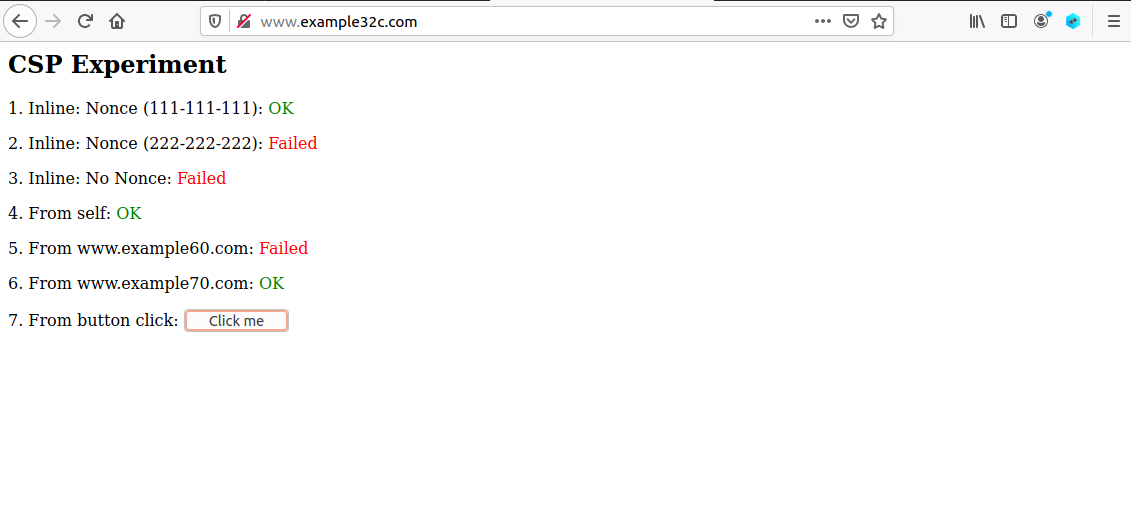
\includegraphics[height=\textheight,width=\textwidth,keepaspectratio]
    {figures/example_c_initial.png}
    \caption{\url{www.example32c.com} initial status.}
    \label{fig:example_c_init}
\end{figure}

\textbf{3. Change the server configuration on \emph{example32b} (modify the Apache
configuration), so Areas 5 and 6 display OK. Please include your modified configuration
in the lab report.}

\begin{lstlisting}[caption=Modified CSP configuration by Apache.,
    label={lst:csp_config_mod_apache}]
    # Purpose: Do not set CSP policies
    <VirtualHost *:80>
    DocumentRoot /var/www/csp
    ServerName www.example32a.com
    DirectoryIndex index.html
    </VirtualHost>
    # Purpose: Setting CSP policies in Apache configuration
    <VirtualHost *:80>
    DocumentRoot /var/www/csp
    ServerName www.example32b.com
    DirectoryIndex index.html
    Header set Content-Security-Policy " \
    default-src 'self'; \
    script-src 'self' *.example70.com *.example60.com\
    "
    </VirtualHost>
    # Purpose: Setting CSP policies in web applications
    <VirtualHost *:80>
    DocumentRoot /var/www/csp
    ServerName www.example32c.com
    DirectoryIndex phpindex.php
    </VirtualHost> 
\end{lstlisting}

\begin{figure}[h]
    \centering
    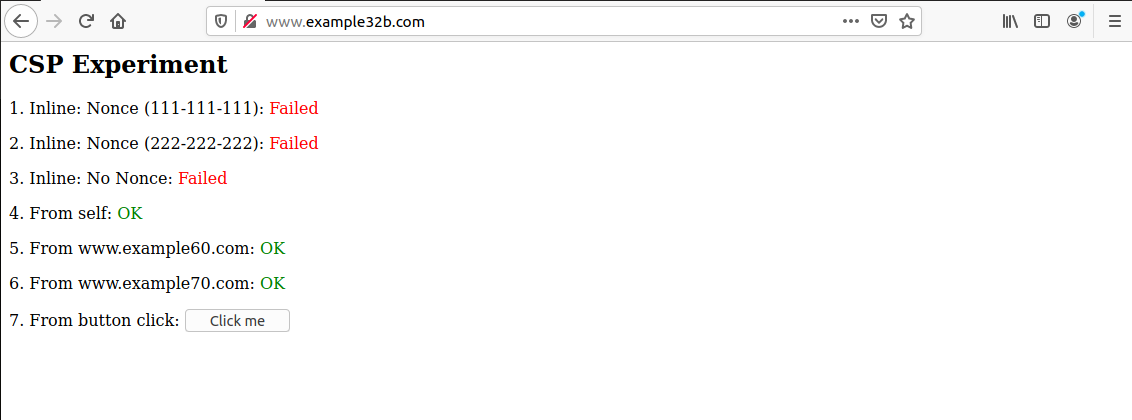
\includegraphics[height=\textheight,width=\textwidth,keepaspectratio]
    {figures/example_b_modified.png}
    \caption{\url{www.example32b.com} status after modifying CSP configuration.}
    \label{fig:example32b_mod}
\end{figure}

To force Area 5 displaying OK, we added \emph{www.exmple60.com} as additional valid source of
external script in the CSP configuration in Apache for \url{www.example32b.com}
(see \autoref{lst:csp_config_mod_apache}). Hence, Area 5 displayed OK (see \autoref{fig:example32b_mod}).
Area 6 displayed OK initially, so we do not need to change anything.

\textbf{4. Change the server configuration on \emph{example32c} (modify the Apache
configuration), so Areas 1,2,4,5, and 6 all display OK. Please include your configuration
in the lab report.}

\begin{lstlisting}[caption=Modified CSP configuration by PHP web application.,
    label={lst:csp_config_mod_php}]
<?php
  $cspheader = "Content-Security-Policy:".
               "default-src 'self';".
               "script-src 'self' 'nonce-111-111-111' 'nonce-222-222-222' *.example60.com *.example70.com".
               "";
  header($cspheader);
?>

<?php include 'index.html';?>
\end{lstlisting}

\begin{figure}[h]
    \centering
    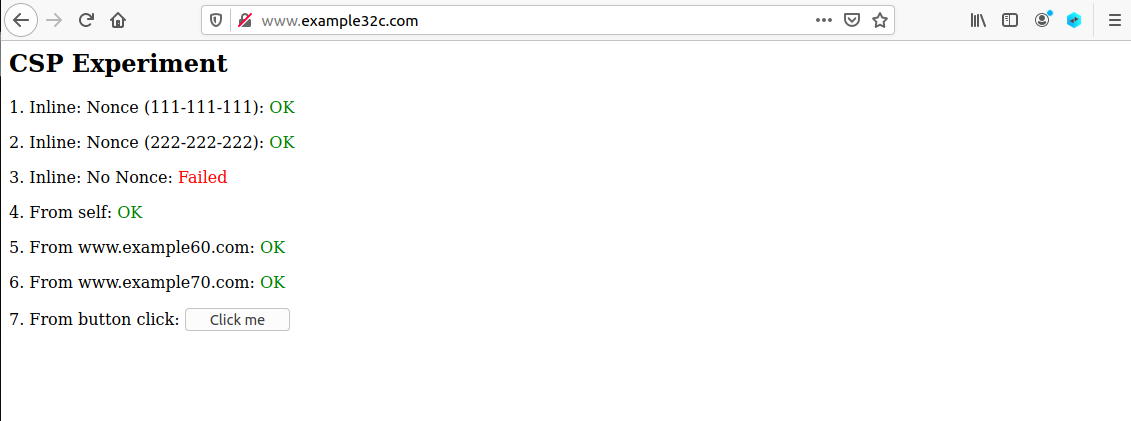
\includegraphics[height=\textheight,width=\textwidth,keepaspectratio]
    {figures/example_c_modified.png}
    \caption{\url{www.example32c.com} status after modifying CSP configuration.}
    \label{fig:example_c_mod}
\end{figure}

With the initial configuration, Areas 1, 4, and 6 displayed OK. To force Areas 2 and 5 displaying
OK, we added the nonce '222-222-222' and URL pattern \url{*.example60.com} to the configuration
file \emph{phpindex.php} (see \autoref{lst:csp_config_mod_php}). Once we rebuilt the container
with the updated configuration, Areas 2 and 5 displayed OK along with 1,4, and 6 (see
\autoref{fig:example_c_mod}).

\textbf{5. Please explain why CSP can help prevent Cross-Site Scripting attacks.}

Cross-Site Scripting attack means that the victim's browser executes malicious
scripts coming from untrusted sources of content~\cite{csp}. So CSP allows server administrators
specify valid sources of executable scripts. Hence, only scripts coming from those
allowed domains are executed, ignoring other highly-potential malicious scripts.